\section{What the certificates rest on}\label{app:restson}

The Qwen certificates rest on questions with exactly zero uncertainty, yet certification does not require them: the Llama-8B receiver agent has none, yet is certified and holds out of sample. Unless marked post hoc, each analysis below ran under rules fixed before computing. The unsaturated-AUROC and receiver-rotation analyses and both unparseable-answer variants are post hoc (Table~\ref{tab:provenance}).

\paragraph{Zero-uncertainty questions among skipped ones.} Over the nine certified Qwen-receiver thresholds, 60.3 to 92.1\% of skipped development questions have $u=0$. These change 0 to 2.2\% of the time, against 3.8 to 20.0\% for the others (Table~\ref{tab:zero_u}; Figure~\ref{fig:zero_u}a). For large/ARC/Text and both large MMLU-Pro policies, the $u>0$ part has a Clopper--Pearson lower bound above 5\%. Thus, their certificates rest on the zeros, and on calibration the $u>0$ part alone would pass at no frozen threshold ($p=0.175$ to $0.999$). For medium/ARC/C2C and medium/OBQA/C2C at $q=0.50$, over 90\% of skipped questions have $u=0$, so contamination \citep{deng2024contamination} could inflate such coverage without voiding a certificate. Out of sample, $u>0$ questions also change more often. On the held-out OBQA questions, 11 of 249 (large Text and C2C), 3 of 82 and 1 of 40 (medium C2C at $q=0.55$ and $0.50$), and 15 of 212 (Text+fact) of the skipped $u>0$ answers change, against 1 to 5 of 306 to 346 zero-uncertainty ones. On the sealed ARC test, every change falls on $u>0$ questions (Text 20 of 263, C2C 11 of 210); none of the 837 zero-uncertainty questions each policy skipped changed. Over all development questions, $u=0$ covers 43.3, 58.2, and 12.3\% for the medium receiver and 47.7, 72.6, and 24.4\% for the large receiver on OBQA, ARC, and MMLU-Pro.

\begin{figure}[!t]\centering
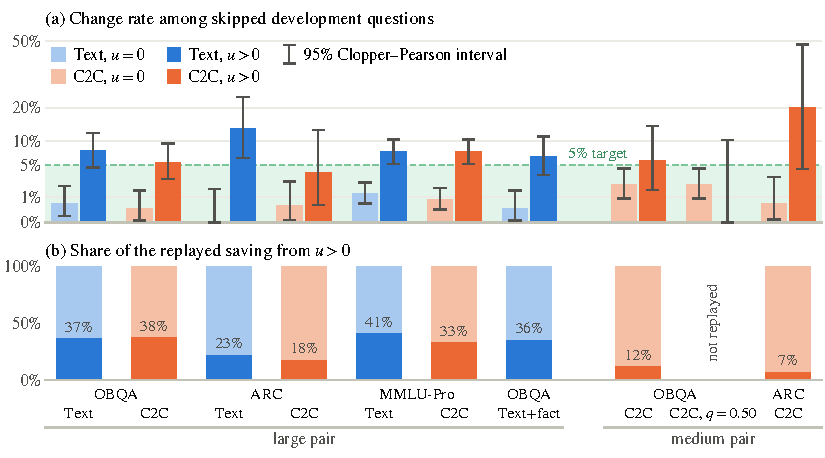
\includegraphics[width=\linewidth]{figures/figure_zero_u.pdf}
\caption{The Qwen certificates rest on zero-uncertainty questions: skipped questions with $u=0$ rarely change, whereas those with $u>0$ change more often and supply 7 to 41\% of the replayed saving. One column per setting in both panels, named below (b). (a)~Change rate among skipped development questions with $u=0$ (light bars) and $u>0$ (dark bars), in the setting's colour (blue: Text and Text+fact; orange: C2C), with two-sided Clopper--Pearson 95\% intervals as whiskers (a rate of 0 has no bar, only its interval), at the nine certified Qwen-receiver thresholds and the medium/OBQA/C2C sensitivity threshold $q=0.50$ (Table~\ref{tab:zero_u}); square-root scale; green band: at or below the 5\% target. (b)~Share of the replayed saving on skipped questions that comes from $u>0$ questions (dark lower part, value printed; light upper part: the $u=0$ share; Table~\ref{tab:u0saving}; not replayed: no replay at $q=0.50$); the Llama-8B receiver (not plotted), which has no $u=0$ question, draws all of its saving from them.}
\label{fig:zero_u}
\end{figure}

\begin{table}[!htbp]\centering\scriptsize
\caption{At the nine deployed thresholds, skipped questions with $u=0$ change 0 to 2.2\% of the time and the others 3.8 to 20.0\% (development). $n$: skipped questions; share: $n_0/n$; $n_0$, $k_0$: skipped questions with $u=0$ and their changes; $n_+$, $k_+$: the others [Clopper--Pearson 95\% CI]. $p_+$: calibration p-value of the $u>0$ part alone (descriptive). Medium/OBQA/C2C is deployed at $q=0.55$; its $q=0.50$ row is a sensitivity threshold, accepted without the parser-review questions (341 calibration questions whose outputs were read with gold labels before the parser was frozen).}
\label{tab:zero_u}
\renewcommand{\arraystretch}{1.1}\setlength{\tabcolsep}{2.5pt}
\begin{tabular*}{\linewidth}{@{}l@{\hspace{5pt}\extracolsep{\fill}}lrcclcll@{}}\toprule
& & & \multicolumn{3}{c}{Skipped questions with $u=0$} & \multicolumn{3}{c}{Skipped questions with $u>0$}\\\cmidrule(lr){4-6}\cmidrule(l){7-9}
Setting & \multicolumn{1}{c}{$q$} & \multicolumn{1}{c}{$n$} & share (\%) & $k_0/n_0$ & \multicolumn{1}{c}{\begin{tabular}[b]{@{}c@{}}change rate (\%)\\{}[95\% CI]\end{tabular}} & $k_+/n_+$ & \multicolumn{1}{c}{\begin{tabular}[b]{@{}c@{}}change rate (\%)\\{}[95\% CI]\end{tabular}} & \multicolumn{1}{c}{\begin{tabular}[b]{@{}c@{}}calibration\\$p_+$\end{tabular}}\\\midrule
large/OBQA/Text & 0.80 & 572 & 61.9 & 2/354 & 0.56 [0.07, 2.03] & 17/218 & 7.80 [4.61, 12.19] & 0.214\\
large/OBQA/C2C & 0.80 & 572 & 61.9 & 1/354 & 0.28 [0.01, 1.56] & 12/218 & 5.50 [2.88, 9.42] & 0.46\\
large/ARC/Text & 0.95 & 284 & 76.4 & 0/217 & 0.00 [0.00, 1.69] & 9/67 & 13.43 [6.33, 23.97] & 0.427\\
large/ARC/C2C & 0.90 & 270 & 80.4 & 1/217 & 0.46 [0.01, 2.54] & 2/53 & 3.77 [0.46, 12.98] & 0.765\\
medium/OBQA/C2C & 0.55 & 390 & 82.3 & 7/321 & 2.18 [0.88, 4.44] & 4/69 & 5.80 [1.60, 14.18] & 0.979\\
medium/OBQA/C2C & 0.50 & 355 & 90.4 & 7/321 & 2.18 [0.88, 4.44] & 0/34 & 0.00 [0.00, 10.28] & 0.601\\
medium/ARC/C2C & 0.60 & 189 & 92.1 & 1/174 & 0.57 [0.01, 3.16] & 3/15 & 20.00 [4.33, 48.09] & 0.175\\
large/MMLU-Pro/Text & 0.40 & 1069 & 60.3 & 8/645 & 1.24 [0.54, 2.43] & 32/424 & 7.55 [5.22, 10.49] & 0.877\\
large/MMLU-Pro/C2C & 0.40 & 1069 & 60.3 & 5/645 & 0.78 [0.25, 1.80] & 32/424 & 7.55 [5.22, 10.49] & 0.999\\
large/OBQA/Text+fact & 0.75 & 536 & 66.0 & 1/354 & 0.28 [0.01, 1.56] & 12/182 & 6.59 [3.45, 11.23] & 0.747\\\bottomrule
\end{tabular*}
\end{table}

\begin{table}[!htbp]\centering\scriptsize
\caption{Without the zero-uncertainty block, ProbeMax still ranks disagreements with development AUROC 0.739 to 0.827. $u>0$: questions with nonzero uncertainty only, with a question-bootstrap 95\% CI and their disagreements / questions; tie-broken: ties broken by the log non-top mass; non-top mass: total probe probability of all labels but the top one; zero block: the $u=0$ questions; within $u=0$: that score inside the zero block (--: no disagreement there); $u=0$: share of questions; disagreements at $u>0$: share of all disagreements.}
\label{tab:auroc_u0}
\renewcommand{\arraystretch}{1.1}\setlength{\tabcolsep}{2.5pt}
\begin{tabular*}{\linewidth}{@{}l@{\hspace{5pt}\extracolsep{\fill}}cccccccc@{}}\toprule
& \multicolumn{4}{c}{Development AUROC} & \multicolumn{2}{c}{Within $u=0$} & & \\\cmidrule(lr){2-5}\cmidrule(lr){6-7}
Policy & all & $u>0$ [95\% CI] & \begin{tabular}[b]{@{}c@{}}disagreements\\/ questions\end{tabular} & tie-broken & AUROC & \begin{tabular}[b]{@{}c@{}}disagreements\\/ questions\end{tabular} & \begin{tabular}[b]{@{}c@{}}$u=0$\\(\%)\end{tabular} & \begin{tabular}[b]{@{}c@{}}Disagreements\\at $u>0$ (\%)\end{tabular}\\\midrule
medium/OBQA/C2C & 0.840 & 0.739 [0.690, 0.789] & 124/421 & 0.848 & 0.777 & 7/321 & 43.3 & 94.7\\
medium/ARC/C2C & 0.910 & 0.748 [0.658, 0.837] & 47/125 & 0.913 & 0.682 & 1/174 & 58.2 & 97.9\\
large/OBQA/Text & 0.873 & 0.769 [0.707, 0.826] & 70/388 & 0.876 & 0.753 & 2/354 & 47.7 & 97.2\\
large/OBQA/C2C & 0.883 & 0.779 [0.724, 0.831] & 59/388 & 0.884 & 0.697 & 1/354 & 47.7 & 98.3\\
large/ARC/Text & 0.952 & 0.796 [0.686, 0.896] & 15/82 & 0.952 & -- & 0/217 & 72.6 & 100\\
large/ARC/C2C & 0.909 & 0.827 [0.673, 0.954] & 11/82 & 0.931 & 0.861 & 1/217 & 72.6 & 91.7\\
large/MMLU-Pro/Text & 0.821 & 0.757 [0.734, 0.778] & 553/1996 & 0.822 & 0.723 & 8/645 & 24.4 & 98.6\\
large/MMLU-Pro/C2C & 0.846 & 0.774 [0.753, 0.795] & 751/1996 & 0.847 & 0.938 & 5/645 & 24.4 & 99.3\\
large/OBQA/Text+fact & 0.889 & 0.781 [0.728, 0.832] & 75/388 & 0.892 & 0.983 & 1/354 & 47.7 & 98.7\\\bottomrule
\end{tabular*}
\end{table}

\paragraph{Ranking without the saturated block.} Post hoc, on $u>0$ questions alone the development AUROC is 0.739 to 0.827 (median 0.774), against a median of 0.883 on all questions, as in Figure~\ref{fig:boundary_map}. With ties broken by the log of the non-top mass, the all-question AUROC is 0.822 to 0.952 (median 0.884; Table~\ref{tab:auroc_u0}); the $u>0$ questions hold 91.7 to 100\% of all disagreements. On the held-out OBQA questions the $u>0$ AUROC is 0.770 to 0.839; the tie-breaking score was not stored there.

\begin{table}[!htbp]\centering\scriptsize
\caption{Skipping exactly the $u=0$ questions passes in every setting ($\tau=0$ is an accepted grid threshold), and the deployed thresholds add skipped questions with $u>0$. Calibration: changed/skipped at $u=0$ and exact binomial p-value; development: coverage and change rate [Clopper--Pearson 95\% CI]. The medium/OBQA/C2C $q=0.50$ row is a sensitivity threshold (deployed: $q=0.55$).}
\label{tab:u0rule}
\renewcommand{\arraystretch}{1.1}\setlength{\tabcolsep}{2pt}
\begin{tabular*}{\linewidth}{@{}l@{\hspace{4pt}\extracolsep{\fill}}lrcccc@{}}\toprule
& \multicolumn{2}{c}{Calibration, $u=0$} & \multicolumn{2}{c}{Development, $u=0$} & \multicolumn{2}{c@{}}{Development, deployed}\\\cmidrule(lr){2-3}\cmidrule(lr){4-5}\cmidrule(l){6-7}
Setting & \multicolumn{1}{c}{$k_0/n_0$} & \multicolumn{1}{c}{$p$} & Coverage (\%) & \begin{tabular}[b]{@{}c@{}}Change rate (\%)\\{}[95\% CI]\end{tabular} & Coverage (\%) & \multicolumn{1}{c@{}}{\begin{tabular}[b]{@{}c@{}}Change rate (\%)\\{}[95\% CI]\end{tabular}}\\\midrule
large/OBQA/Text & 1/642 & $1.7\times10^{-13}$ & 47.7 & 0.56 [0.07, 2.03] & 77.1 & 3.32 [2.01, 5.14]\\
large/OBQA/C2C & 2/642 & $3.0\times10^{-12}$ & 47.7 & 0.28 [0.01, 1.56] & 77.1 & 2.27 [1.22, 3.86]\\
large/ARC/Text & 0/321 & $7.1\times10^{-8}$ & 72.6 & 0.00 [0.00, 1.69] & 95.0 & 3.17 [1.46, 5.93]\\
large/ARC/C2C & 2/321 & $1.1\times10^{-5}$ & 72.6 & 0.46 [0.01, 2.54] & 90.3 & 1.11 [0.23, 3.21]\\
large/MMLU-Pro/Text & 14/1442 & $2.1\times10^{-17}$ & 24.4 & 1.24 [0.54, 2.43] & 40.5 & 3.74 [2.69, 5.06]\\
large/MMLU-Pro/C2C & 9/1442 & $1.9\times10^{-21}$ & 24.4 & 0.78 [0.25, 1.80] & 40.5 & 3.46 [2.45, 4.74]\\
medium/OBQA/C2C ($q=0.55$) & 7/601 & $3.2\times10^{-7}$ & 43.3 & 2.18 [0.88, 4.44] & 52.6 & 2.82 [1.42, 4.99]\\
medium/OBQA/C2C ($q=0.50$) & 7/601 & $3.2\times10^{-7}$ & 43.3 & 2.18 [0.88, 4.44] & 47.8 & 1.97 [0.80, 4.02]\\
medium/ARC/C2C & 1/256 & $2.9\times10^{-5}$ & 58.2 & 0.57 [0.01, 3.16] & 63.2 & 2.12 [0.58, 5.33]\\
large/OBQA/Text+fact & 2/642 & $3.0\times10^{-12}$ & 47.7 & 0.28 [0.01, 1.56] & 72.2 & 2.43 [1.30, 4.11]\\\bottomrule
\end{tabular*}
\end{table}

\paragraph{Skipping exactly the zero-uncertainty questions.} In all nine settings, several low grid quantiles coincide at $\tau=0$ and that threshold is accepted. Therefore, the rule that skips a question if and only if $u=0$ was among the tested candidates (Table~\ref{tab:u0rule}). On development, it skips 24.4 to 72.6\% of questions and changes 0 to 2.2\% of them, against 40.5 to 95.0\% and 1.1 to 3.7\% for the deployed thresholds. With fit, calibration, and development restricted to $u>0$ questions and fit quantiles taken over them, the test certifies 1 of 9 settings: large/OBQA/C2C ($q=0.35$; 3 of 257 calibration questions change, $p=9.7\times10^{-4}$; 16.4\% of development questions skipped, 1 of 122 changed). The others fall back (smallest $p$ from 0.002 to 0.60).

\begin{table}[!htbp]\centering\scriptsize
\caption{Skipped questions with $u>0$ supply 7.3 to 41.3\% of the saving on skipped questions for the eight Qwen-receiver policies whose interval excludes zero, and all of it for the Llama-8B receiver. Paired mean saving (ms) by source, and the number $n$ of questions from each source, over the 128-question panels (Llama-8B and Text+fact on the second configuration, all others on the original one) and, $^\ast$, over the full 2,641-question MMLU-Pro C2C replay (second configuration); ms: each source's contribution to Saving; Routed: questions sent to the reference; Share: $u>0$ part over the skipped parts; Recomposed: saving if only $u=0$ questions were skipped.}
\label{tab:u0saving}
\renewcommand{\arraystretch}{1.1}\setlength{\tabcolsep}{2pt}
\begin{tabular*}{\linewidth}{@{}l@{\hspace{5pt}\extracolsep{\fill}}rrrrrrcrc@{}}\toprule
& \multicolumn{2}{c}{Skipped, $u=0$} & \multicolumn{2}{c}{Skipped, $u>0$} & \multicolumn{2}{c}{Routed} & & & \\\cmidrule(lr){2-3}\cmidrule(lr){4-5}\cmidrule(lr){6-7}
Policy & ms & $n$ & ms & $n$ & ms & $n$ & \begin{tabular}[b]{@{}c@{}}Saving (ms)\\{}[95\% CI]\end{tabular} & \begin{tabular}[b]{@{}c@{}}Share\\from $u>0$\end{tabular} & \begin{tabular}[b]{@{}c@{}}Recomposed (ms)\\{}[95\% CI]\end{tabular}\\\midrule
large/OBQA/Text & 332.9 & 60 & 194.5 & 37 & $-10.3$ & 31 & 517.1 [447.8, 583.6] & 0.369 & 294.9 [211.5, 372.4]\\
large/OBQA/C2C & 29.1 & 60 & 17.7 & 37 & $-10.2$ & 31 & 36.6 [18.0, 56.8] & 0.378 & 6.7 [$-9.5$, $+24.8$]\\
large/ARC/Text & 557.3 & 93 & 163.1 & 27 & $-2.8$ & 8 & 717.6 [670.6, 763.2] & 0.226 & 545.6 [476.1, 614.0]\\
large/ARC/C2C & 94.7 & 93 & 20.5 & 22 & $-4.2$ & 13 & 110.9 [82.0, 142.8] & 0.178 & 83.2 [55.2, 111.0]\\
large/MMLU-Pro/Text & 204.5 & 30 & 144.0 & 18 & $-2.2$ & 80 & 346.3 [249.8, 443.0] & 0.413 & 196.0 [113.6, 287.0]\\
large/MMLU-Pro/C2C & 23.2 & 30 & 11.6 & 18 & $-26.6$ & 80 & 8.2 [$-20.5$, $+44.0$] & 0.334 & $-9.8$ [$-33.7$, $+17.9$]\\
medium/OBQA/C2C & 67.0 & 55 & 9.4 & 11 & 3.2 & 62 & 79.7 [48.1, 129.1] & 0.123 & 67.4 [35.6, 115.2]\\
medium/ARC/C2C & 105.6 & 70 & 8.3 & 7 & $-13.3$ & 51 & 100.7 [74.5, 133.1] & 0.073 & 90.5 [63.5, 123.1]\\
large/OBQA/Text+fact & 224.5 & 60 & 124.3 & 32 & $-5.3$ & 36 & 343.4 [297.7, 386.0] & 0.356 & 211.2 [162.0, 258.0]\\
Llama-8B/OBQA/Text & 0.0 & 0 & 337.6 & 76 & $-19.0$ & 52 & 318.6 [261.1, 372.1] & 1.000 & $-37.7$ [$-48.3$, $-31.7$]\\
Llama-8B/ARC/Text & 0.0 & 0 & 427.3 & 88 & $-8.4$ & 40 & 418.9 [361.7, 473.7] & 1.000 & $-30.8$ [$-33.4$, $-27.8$]\\
\midrule
large/MMLU-Pro/C2C$^\ast$ & 35.9 & 645 & 12.1 & 424 & $-24.6$ & 1572 & 23.3 [14.5, 32.2] & 0.252 & 4.5 [$-2.9$, $+12.1$]\\\bottomrule
\end{tabular*}
\end{table}

\paragraph{Where the replayed saving comes from.} Splitting each replayed policy's paired mean saving by source, using the scores and routes logged by each policy request, skipped questions with $u>0$ supply 7.3 to 41.3\% of the saving on skipped questions among the eight Qwen-receiver policies whose interval excludes zero (33.4\% for large/MMLU-Pro/C2C). The Llama-8B receiver, which has no $u=0$ question, draws its whole saving from them (Table~\ref{tab:u0saving}; Figure~\ref{fig:zero_u}b). A recomposed rule that skips only the $u=0$ questions, charging each other skipped question its fixed latency plus its logged probe time, would keep 57 to 76\% of the Text savings, 75\% of the large/ARC/C2C saving, 18\% of the large/OBQA/C2C saving, and 85 to 90\% of the medium-pair savings. It would not save for large/MMLU-Pro/C2C ($-9.8$~ms).

\begin{table}[!htbp]\centering\scriptsize
\caption{At $u=0$, option rotation changes the medium and large receivers' own answers 1.8 to 6.3\% of the time, against 19.5 to 44.6\% at $u>0$ (receiver alone, development) [Clopper--Pearson 95\% CI]. Option rotation: each option's text moved one position down, labels kept (answers mapped back). Change rate: Changed$/n$, not a policy's change rate. Both answers parse: changed answers out of the questions on which both the original and the rotated answer parse; --: no question.}
\label{tab:rot_dev}
\renewcommand{\arraystretch}{1.1}\setlength{\tabcolsep}{2pt}
\begin{tabular*}{\linewidth}{@{}l@{\hspace{6pt}}l@{\hspace{4pt}\extracolsep{\fill}}rclrclc@{}}\toprule
& & \multicolumn{3}{c}{Development questions with $u=0$} & \multicolumn{3}{c}{Development questions with $u>0$} & \\\cmidrule(lr){3-5}\cmidrule(lr){6-8}
Receiver & Task & \multicolumn{1}{c}{$n$} & Changed & \multicolumn{1}{c}{\begin{tabular}[b]{@{}c@{}}Change rate (\%)\\{}[95\% CI]\end{tabular}} & \multicolumn{1}{c}{$n$} & Changed & \multicolumn{1}{c}{\begin{tabular}[b]{@{}c@{}}Change rate (\%)\\{}[95\% CI]\end{tabular}} & \multicolumn{1}{c@{}}{\begin{tabular}[b]{@{}c@{}}Both answers parse:\\changed / questions\end{tabular}}\\\midrule
small & OBQA & 0 & -- & \multicolumn{1}{c}{--} & 742 & 558 & 75.2 [71.9, 78.3] & 521/696\\
small & ARC & 0 & -- & \multicolumn{1}{c}{--} & 299 & 209 & 69.9 [64.4, 75.0] & 180/258\\
medium & OBQA & 321 & 19 & 5.9 [3.6, 9.1] & 421 & 164 & 39.0 [34.3, 43.8] & 176/732\\
medium & ARC & 174 & 11 & 6.3 [3.2, 11.0] & 125 & 42 & 33.6 [25.4, 42.6] & 51/297\\
large & OBQA & 354 & 9 & 2.5 [1.2, 4.8] & 388 & 128 & 33.0 [28.3, 37.9] & 134/739\\
large & ARC & 217 & 4 & 1.8 [0.5, 4.7] & 82 & 16 & 19.5 [11.6, 29.7] & 20/299\\
large & MMLU-Pro & 645 & 23 & 3.6 [2.3, 5.3] & 1996 & 891 & 44.6 [42.4, 46.9] & 906/2631\\\bottomrule
\end{tabular*}
\end{table}

\paragraph{Option order.} Post hoc, rotating the options as in the null control (answers mapped back) changes the medium and large receivers' own $u=0$ development answers 1.8 to 6.3\% of the time, against 19.5 to 44.6\% at $u>0$. The upper bound at $u=0$ exceeds 5\% for medium OBQA (9.1\%), medium ARC (11.0\%), and large MMLU-Pro (5.3\%), so part of the receiver's confident answers follow option position (Table~\ref{tab:rot_dev}). These are changes of the receiver's own answer, not a policy's change rate. On each policy's skipped development questions, the receiver's answer changes under rotation 3.3 to 10.0\% of the time. In contrast, the five rotated large-pair policies change 1.7 to 2.6\% of skipped answers relative to their rotated references (Table~\ref{tab:rotation}). The rotated receiver-only runs stored no probe score.

\paragraph{Precision and ties.} At an exact zero, every non-top label has probability below $2^{-24}$ and all of them together below $2^{-23}$ (at most $1.08\times10^{-7}$). Recomputing the probe in FP32 (where 48 and 72\% of the large receiver's OBQA and ARC questions, and 45 and 57\% of the medium receiver's, stay exactly zero, and development coverage moves by at most 0.94 points), or breaking ties by the log of the non-top mass, changes no certification decision in 23 settings. By contrast, the top-two logit gap, itself tied on 98 to 100\% of questions, moves medium/OBQA/C2C to $q=0.50$. No setting switches between deployment and fallback under either score.

\paragraph{Unparseable answers.} A question counts as a disagreement when exactly one of the two answers fails to parse. These make up 0.000 to 0.707 of disagreement across the 18 main settings (pooled 0.274 on calibration and 0.264 on development) and 0.187 to 0.495 across the seven OLMo and Llama settings. Post hoc, in separate 20-test families with unchanged fit thresholds, a non-deployable filter keeping only questions where both answers parse leaves all 11 certified multiple-choice policies at their quantile. It also certifies the three OLMo settings and medium/MMLU-Pro/C2C ($q=0.15$). A deployable rule that routes to the reference whenever the receiver's own answer fails to parse changes no outcome. Every development change of the large-pair OBQA and ARC, Text+fact, and Llama-8B policies is between parsed answers, as is every change on the sealed test, for Text+fact held out, and in the two Llama-8B tests. Exactly one \textsc{invalid} answer is involved in 2 of 40 and 3 of 37 development changes for the two MMLU-Pro policies and 2 of 11 for medium/OBQA/C2C, and out of sample in 1 of 12 and 2 of 13 held-out changes for large/OBQA/Text and C2C and 2 of 8 for medium/OBQA/C2C. For medium/ARC/C2C, 2 of 4 development and 7 of 15 out-of-sample changes involve a C2C answer that does not parse.
